\chapter{Métodos de Kernel}
\label{CAP2}


Este capítulo tem como objetivo 


\section{Kernel em análise de padrões}\label{Sub:equa}

Em análise de padrões, temos como objetivo detectar automaticamente padrões em um conjunto de dados de um determinado problema. Por padrões, podemos entender qualquer relação ou regularidades inerentes à alguma estrutura em uma fonte de dados. Essa análise geralmente é feita a partir dos valores de entrada e suas respectivas saídas(no caso da aprendizagem supervisionada) fornecidas no problema. Essas informações podem formar padrões em que se torna possível verificar o valor de uma saída dada uma nova entrada fornecida pelo usuário. 

Diversos problemas podem ser resolvidos utilizando esta abordagem, categorização de textos, análise de sequências de DNA, reconhecimento de escrita, por exemplo.

A abordagem de análise de padrões utilizando métodos de kernel se baseia em adaptar os dados de entrada em um espaço característico adequado e nos algoritmos usados para descobrir os padrões do problema. Levando em conta isso, podemos pensar que qualquer solução com métodos de kernel é composta por estas duas partes: uma em que é feito o mapeamento nesse espaço característico e a outra em que é executado o algoritmo de aprendizagem para detectar os padrões neste espaço. A ideia por trás desta abordagem é poder mapear os dados em um espaço em que possamos 

Uma das principais caracerísticas desses métodos é o atalho computacional que pode ser utilizado, tal atalho é conhecido como função de kernel.


O Kernel  é uma função de mapeamento de dados em dimensões superiores com a motivação de torná-los mais fáceis de separar ou estruturá-los de maneira mais adequada. Essas funções podem ser utilizadas nas tarefas de reconhecimento de padrões. 

\begin{equation}\label{Eq:multiplicacao}
%
Z = X \cdot Y,
%
\end{equation}
%
em que $Z$, $X$ e $Y$ são variáveis complexas. A referenciação à Equação (\ref{Eq:multiplicacao}) é feita por meio do comando ``ref''. O mesmo vale para outros tipos de elementos.

\subsection{Exemplo de uma equação mais complexa}

  Equações mais complexas podem ser mais facilmente escritas com uso do programa TexAide. Como, por exemplo,

    \begin{equation}\label{Eq:sqrt_gamma_X}
    f_{\Gamma ^{{1 \mathord{\left/
    {\vphantom {1 2}} \right.
    \kern-\nulldelimiterspace} 2}} } (x;\alpha ,\lambda ) = \frac{{2\lambda ^\alpha  }}{{\Gamma (\alpha )}}x^{2\alpha  - 1} \exp \left( { - \lambda x^2 } \right).
    \end{equation}
    \[
    \alpha ,\lambda > 0.
    \]
    %
    em que $\Gamma(\cdot)$ é a função Gama. O programa TexAide é semelhante ao \textit{MathType} do Office, porém ao copiar e colar a equação em um arquivo tex, é gerado o código em LaTex referente a esta equação.

\section{Tabelas}

Tabelas são essenciais na apresentação de dados. A Tabela \ref{Tb:X_models} mostra um exemplo do uso deste tipo de elemento. Vale ressaltar que não é aconselhável o uso de linhas verticais em trabalhos acadêmicos e de pesquisa.

\begin{table}[h]
 \caption{Modelos estatísticos e suas relações.}%
 \label{Tb:X_models}
  \centering
\begin{tabular}{c c c c c}
 \hline
 &&&&\\
                                             &$\alpha ,\lambda  > 0$    &                               &$\alpha ,\lambda \rightarrow\infty$  &Homogêneo \\
                                             &$\gamma  \to 0$           & Heterogêneo                   &$\alpha / \lambda \rightarrow \beta$ & \\
                                             &$\mathop  \to \limits^D $ & $\sqrt\Gamma(\alpha,\lambda)$ &$\mathop  \to \limits^P $            &$\sqrt\beta$        \\
$\mathcal{N}^{-1/2}(x;\alpha,\gamma,\lambda)$& & & &\\
                                             &$\mathop  \to \limits^D $ & $\Gamma^{-1/2}(\alpha,\gamma)$&$\mathop  \to \limits^P $   &$\sqrt{\zeta^{-1}}$ \\
                                             &$\lambda \to 0$           &  Extremamente                 &$-\alpha / \gamma \rightarrow \zeta^{-1}$ & \\
                                             &$-\alpha ,\gamma   > 0$   &  Heterogêneo                  &$-\alpha ,\gamma \rightarrow\infty$ &Homogêneo \\
 &&&& \\
 \hline
 &&&&\\
                                             &$\alpha ,\lambda  > 0$    &                               &$\alpha ,\lambda \rightarrow\infty$  &Homogêneo \\
                                             &$\gamma  \to 0$           & Heterogêneo                   &$\alpha / \lambda \rightarrow \beta$ & \\
                                             &$\mathop  \to \limits^D $ &$\mathcal{K}_A(\alpha,\lambda,n)$&$\mathop  \to \limits^P $&$\sqrt\Gamma(n,n/\beta)$        \\
$\mathcal{G}_A(z;\alpha,\gamma,\lambda,n)$   & & & &\\
                                             &$\mathop  \to \limits^D $ & $\mathcal{G}_A^0(\alpha,\gamma,n)$&$\mathop  \to \limits^P $&$\sqrt\Gamma(n,n\zeta)$  \\
                                             &$\lambda \to 0$           &  Extremamente                 &$-\alpha / \gamma \rightarrow \zeta$ & \\
                                             &$-\alpha ,\gamma   > 0$   &  Heterogêneo                  &$-\alpha ,\gamma \rightarrow\infty$ &Homogêneo \\
&&&&   \\
 \hline

\end{tabular}
\end{table}


A Figura \ref{Fig:1} mostra o exemplo do uso do comando ``subfigure''. Apesar de aceitar diferentes tipos de imagens. É preferível que as imagens estejam no formato .eps. Isso garante que a imagem impressa seja exatamente aquela visualizada, como acontece com arquivos pdf.

\begin{figure}[!ht]
\centering
\subfloat[]{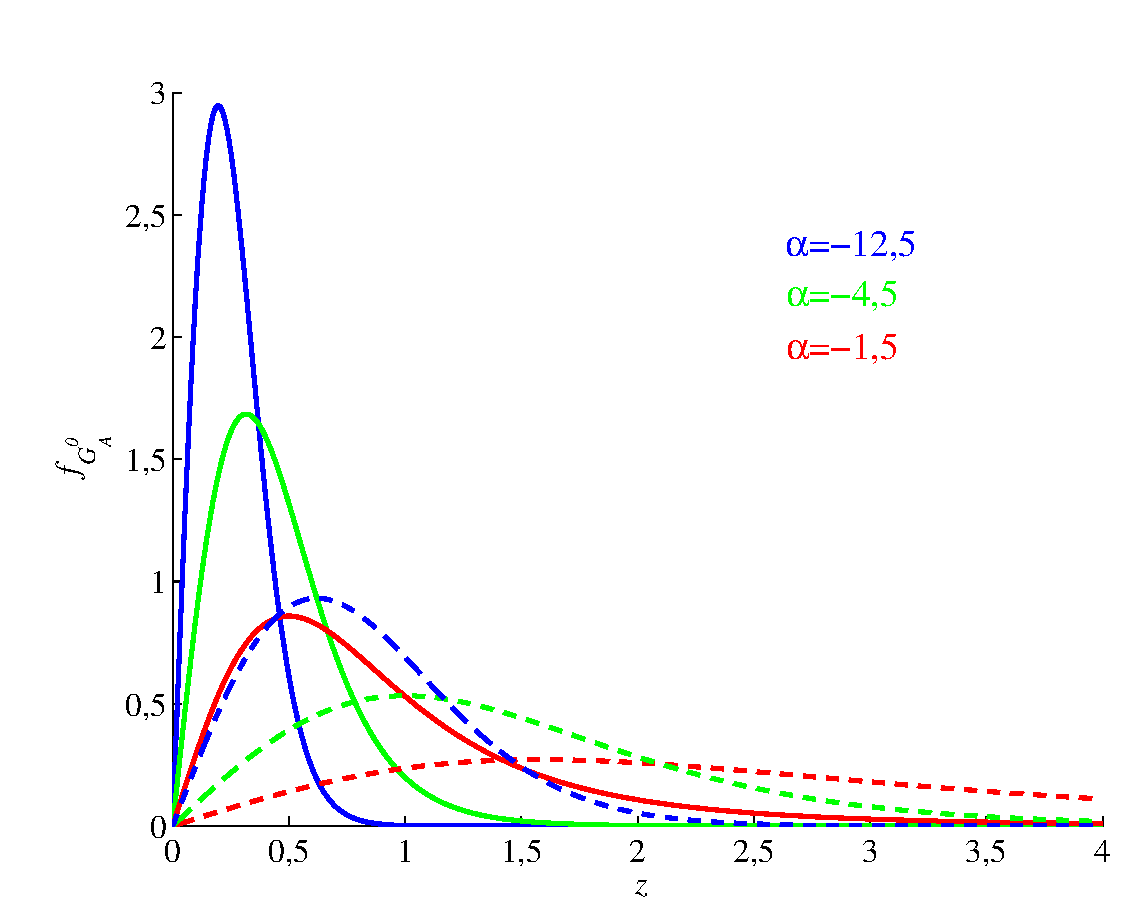
\includegraphics[scale=.65]{figures/fig1.eps}}\\
\subfloat[]{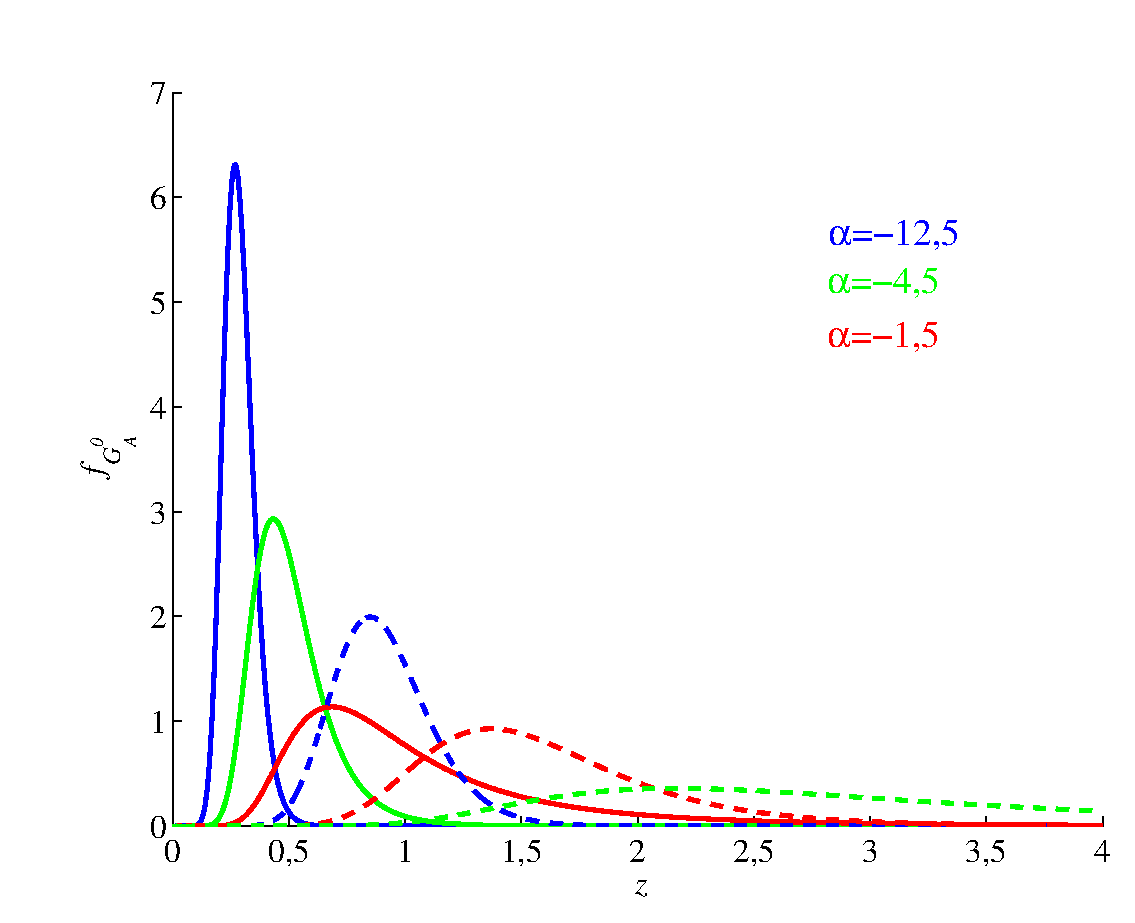
\includegraphics[scale=.65]{figures/fig2.eps}}
\caption{ Curvas de funções de probabilidade: (a) exemplo 1, (b) exemplo 2.} \label{Fig:1}
\end{figure}